\documentclass[12pt]{article}

\usepackage[a4paper, margin=1in]{geometry}

\usepackage{listings}
\usepackage{color}
\usepackage{float}
\usepackage{graphicx}
\usepackage{subcaption}

\definecolor{codegreen}{rgb}{0,0.6,0}
\definecolor{codegray}{rgb}{0.5,0.5,0.5}
\definecolor{codepurple}{rgb}{0.58,0,0.82}
\definecolor{backcolour}{rgb}{0.95,0.95,0.92}

\lstdefinestyle{mystyle}{
  backgroundcolor=\color{backcolour},
  commentstyle=\color{codegreen},
  keywordstyle=\color{magenta},
  numberstyle=\tiny\color{codegray},
  stringstyle=\color{codepurple},
  basicstyle=\ttfamily,
  breakatwhitespace=false,
  breaklines=true,
  captionpos=b,
  keepspaces=true,
  numbers=left,
  numbersep=5pt,
  showspaces=false,
  showstringspaces=false,
  showtabs=false,
  tabsize=2
}

\lstset{style=mystyle}

\setlength\parindent{0pt}
\setlength\parskip{1em}

\title{\vspace{-1.5cm}Lab 8 - Scatter}
\author{\textsc{Nguyen} Duc Tung}
\date{}

\begin{document}

\maketitle

In this labwork, I implemented a RGB to HSV conversion, and a HSV to RGB conversion. Each pixel is converted using the given formula. The kernel's reliability is checked by switching the image back and forth between RGB and HSV without changing the image.

There is no dedicated optimization for Scatter yet. But I just tweaked a bit on the if/else to avoid 1 branch divergent.

\begin{lstlisting}[language=C]
if (delta == 0) {
    hue = 0;
    saturation = 0;
} else {
    saturation = delta / max;

    if (max == R) {
        hue = 60 * (((G - B) / delta) % 6);
    } else if (max == G) {
        hue = 60 * ((B - R) / delta + 2);
    } else {
        hue = 60 * ((R - G) / delta + 4);
    }
}
\end{lstlisting}

instead of

\begin{lstlisting}[language=C]
if (max == 0) {
    saturation = 0;
} else {
    saturation = delta / max;
}

if (delta == 0) {
    hue = 0;
} else {
    if (max == R) {
        hue = 60 * (((G - B) / delta) % 6);
    } else if (max == G) {
        hue = 60 * ((B - R) / delta + 2);
    } else {
        hue = 60 * ((R - G) / delta + 4);
    }
}
\end{lstlisting}

The image remains the same before and after doing color space conversion.

Time elapsed: 27.5 ms

\begin{figure}[H]
  \centering
  \begin{subfigure}{.45\textwidth}
    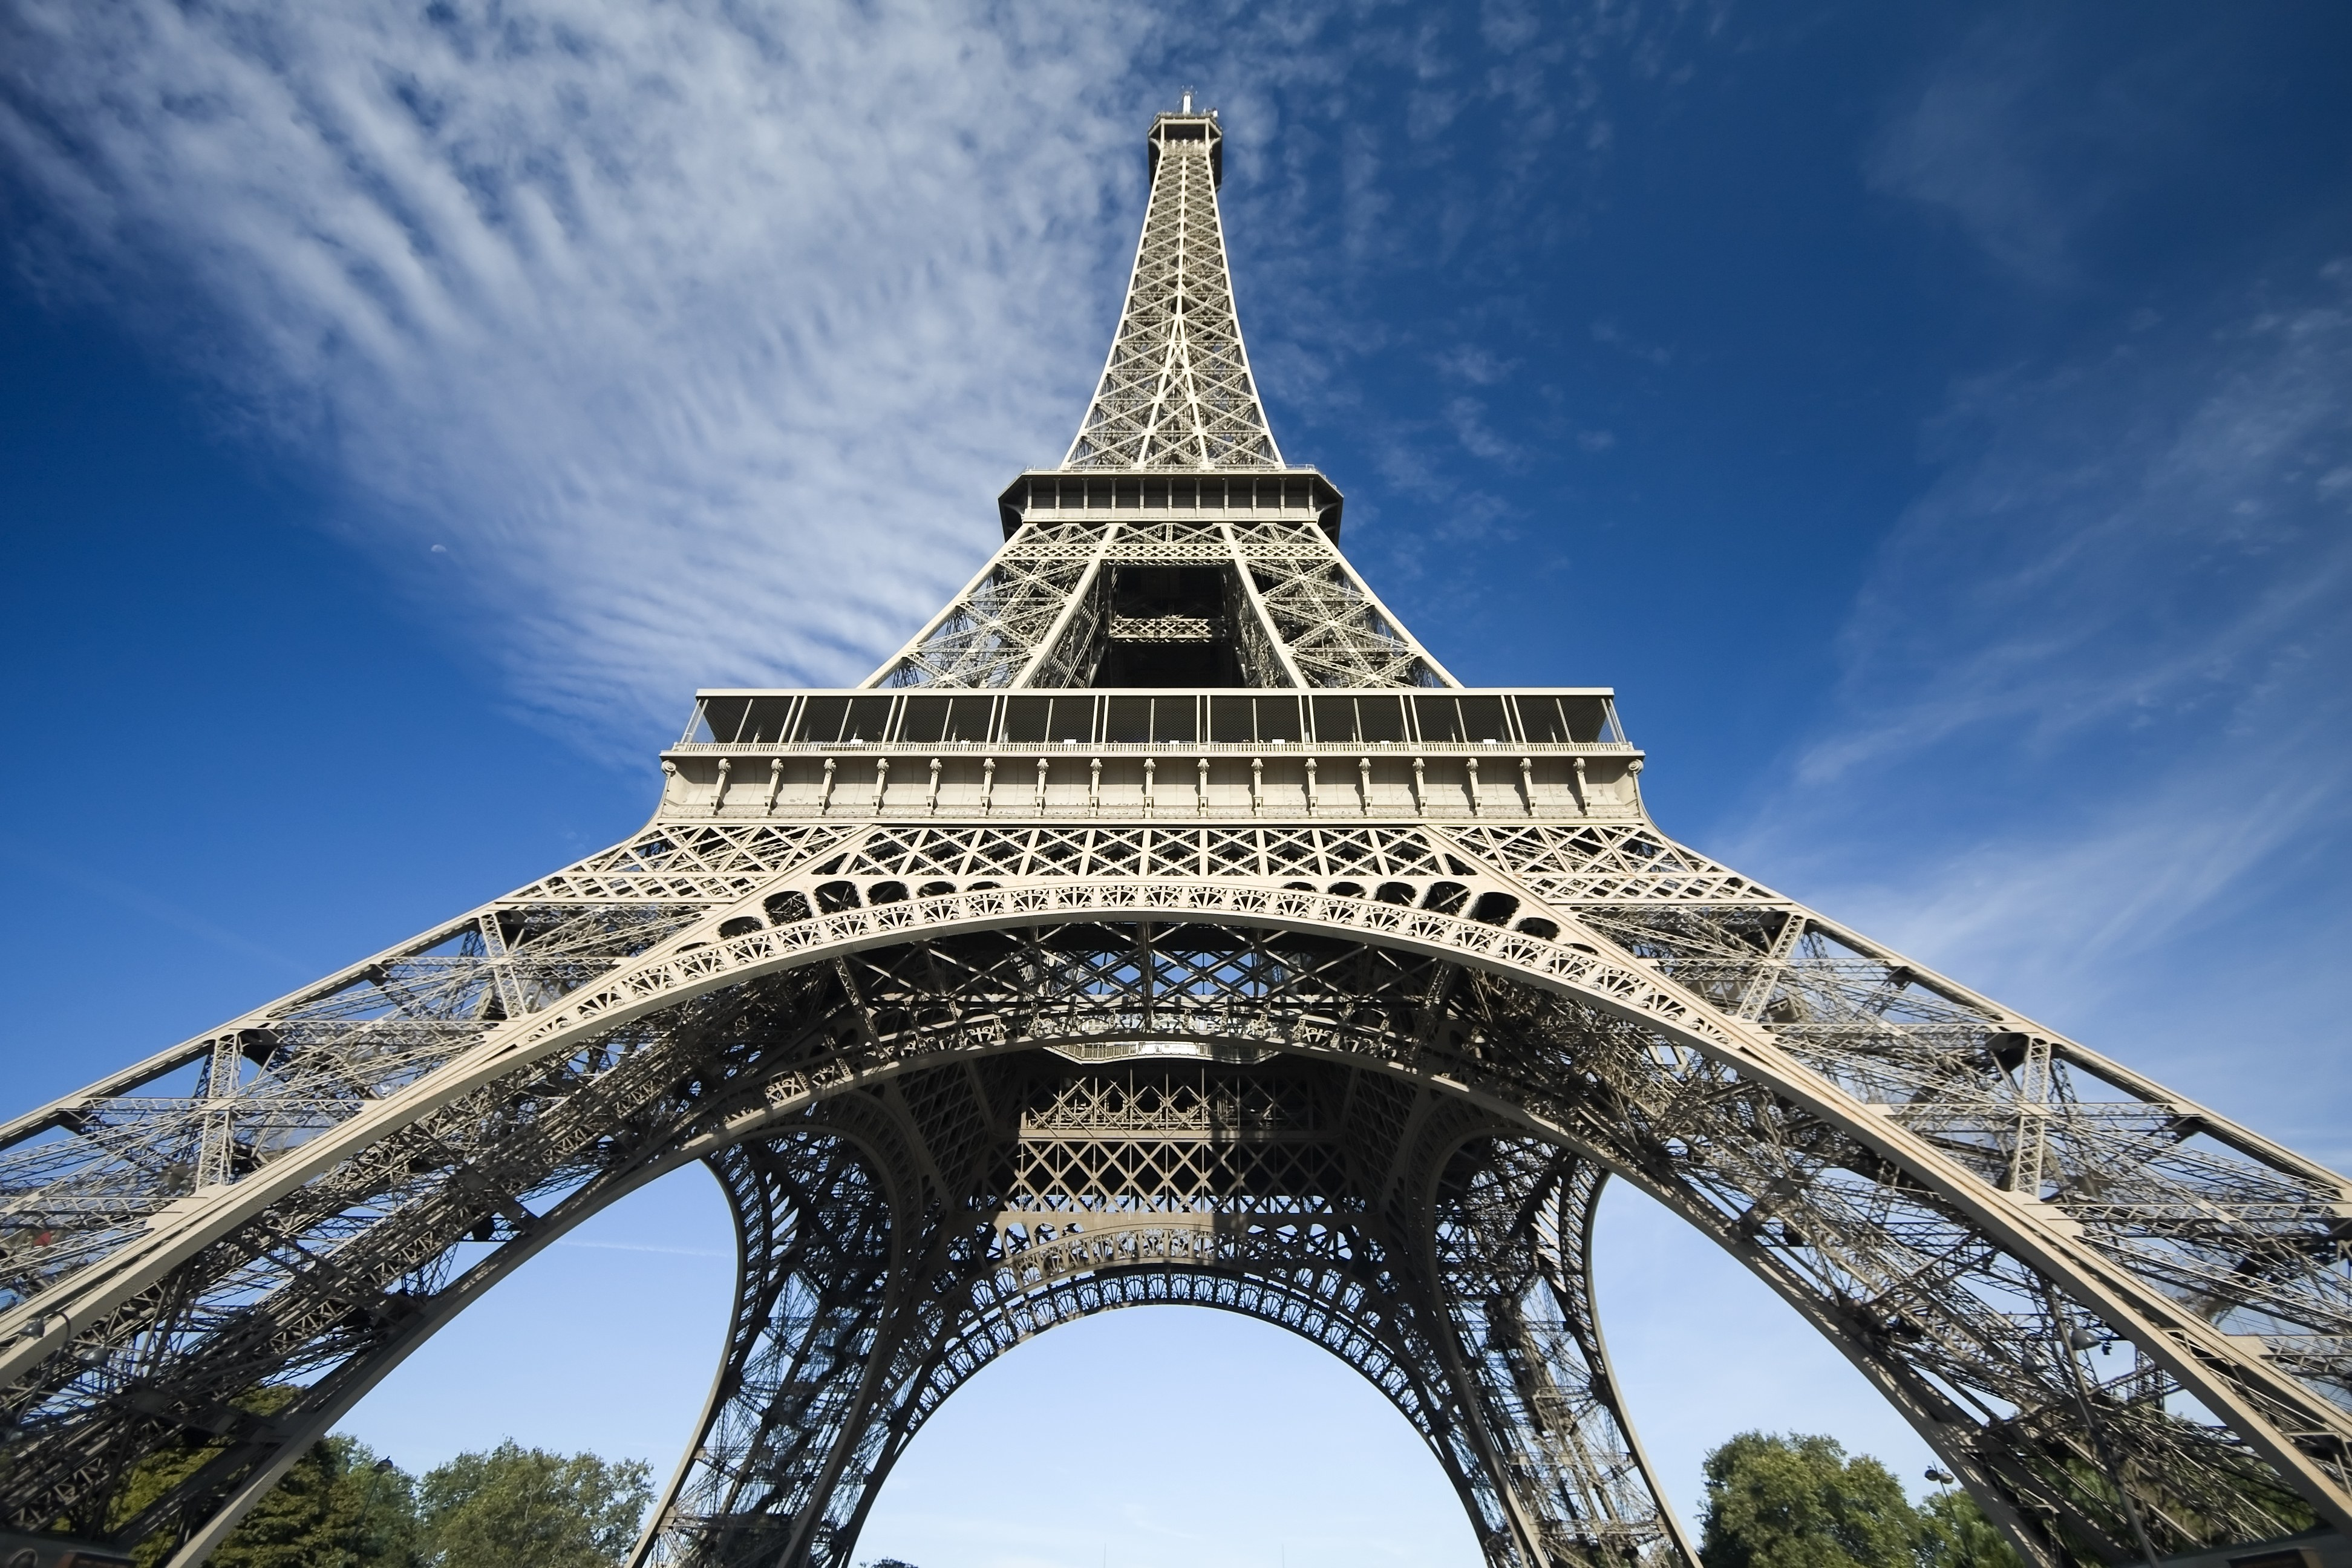
\includegraphics[width=\linewidth]{./img/in.jpg}
    \caption{Original image}
  \end{subfigure}
  \hspace{1cm}
  \begin{subfigure}{.45\textwidth}
    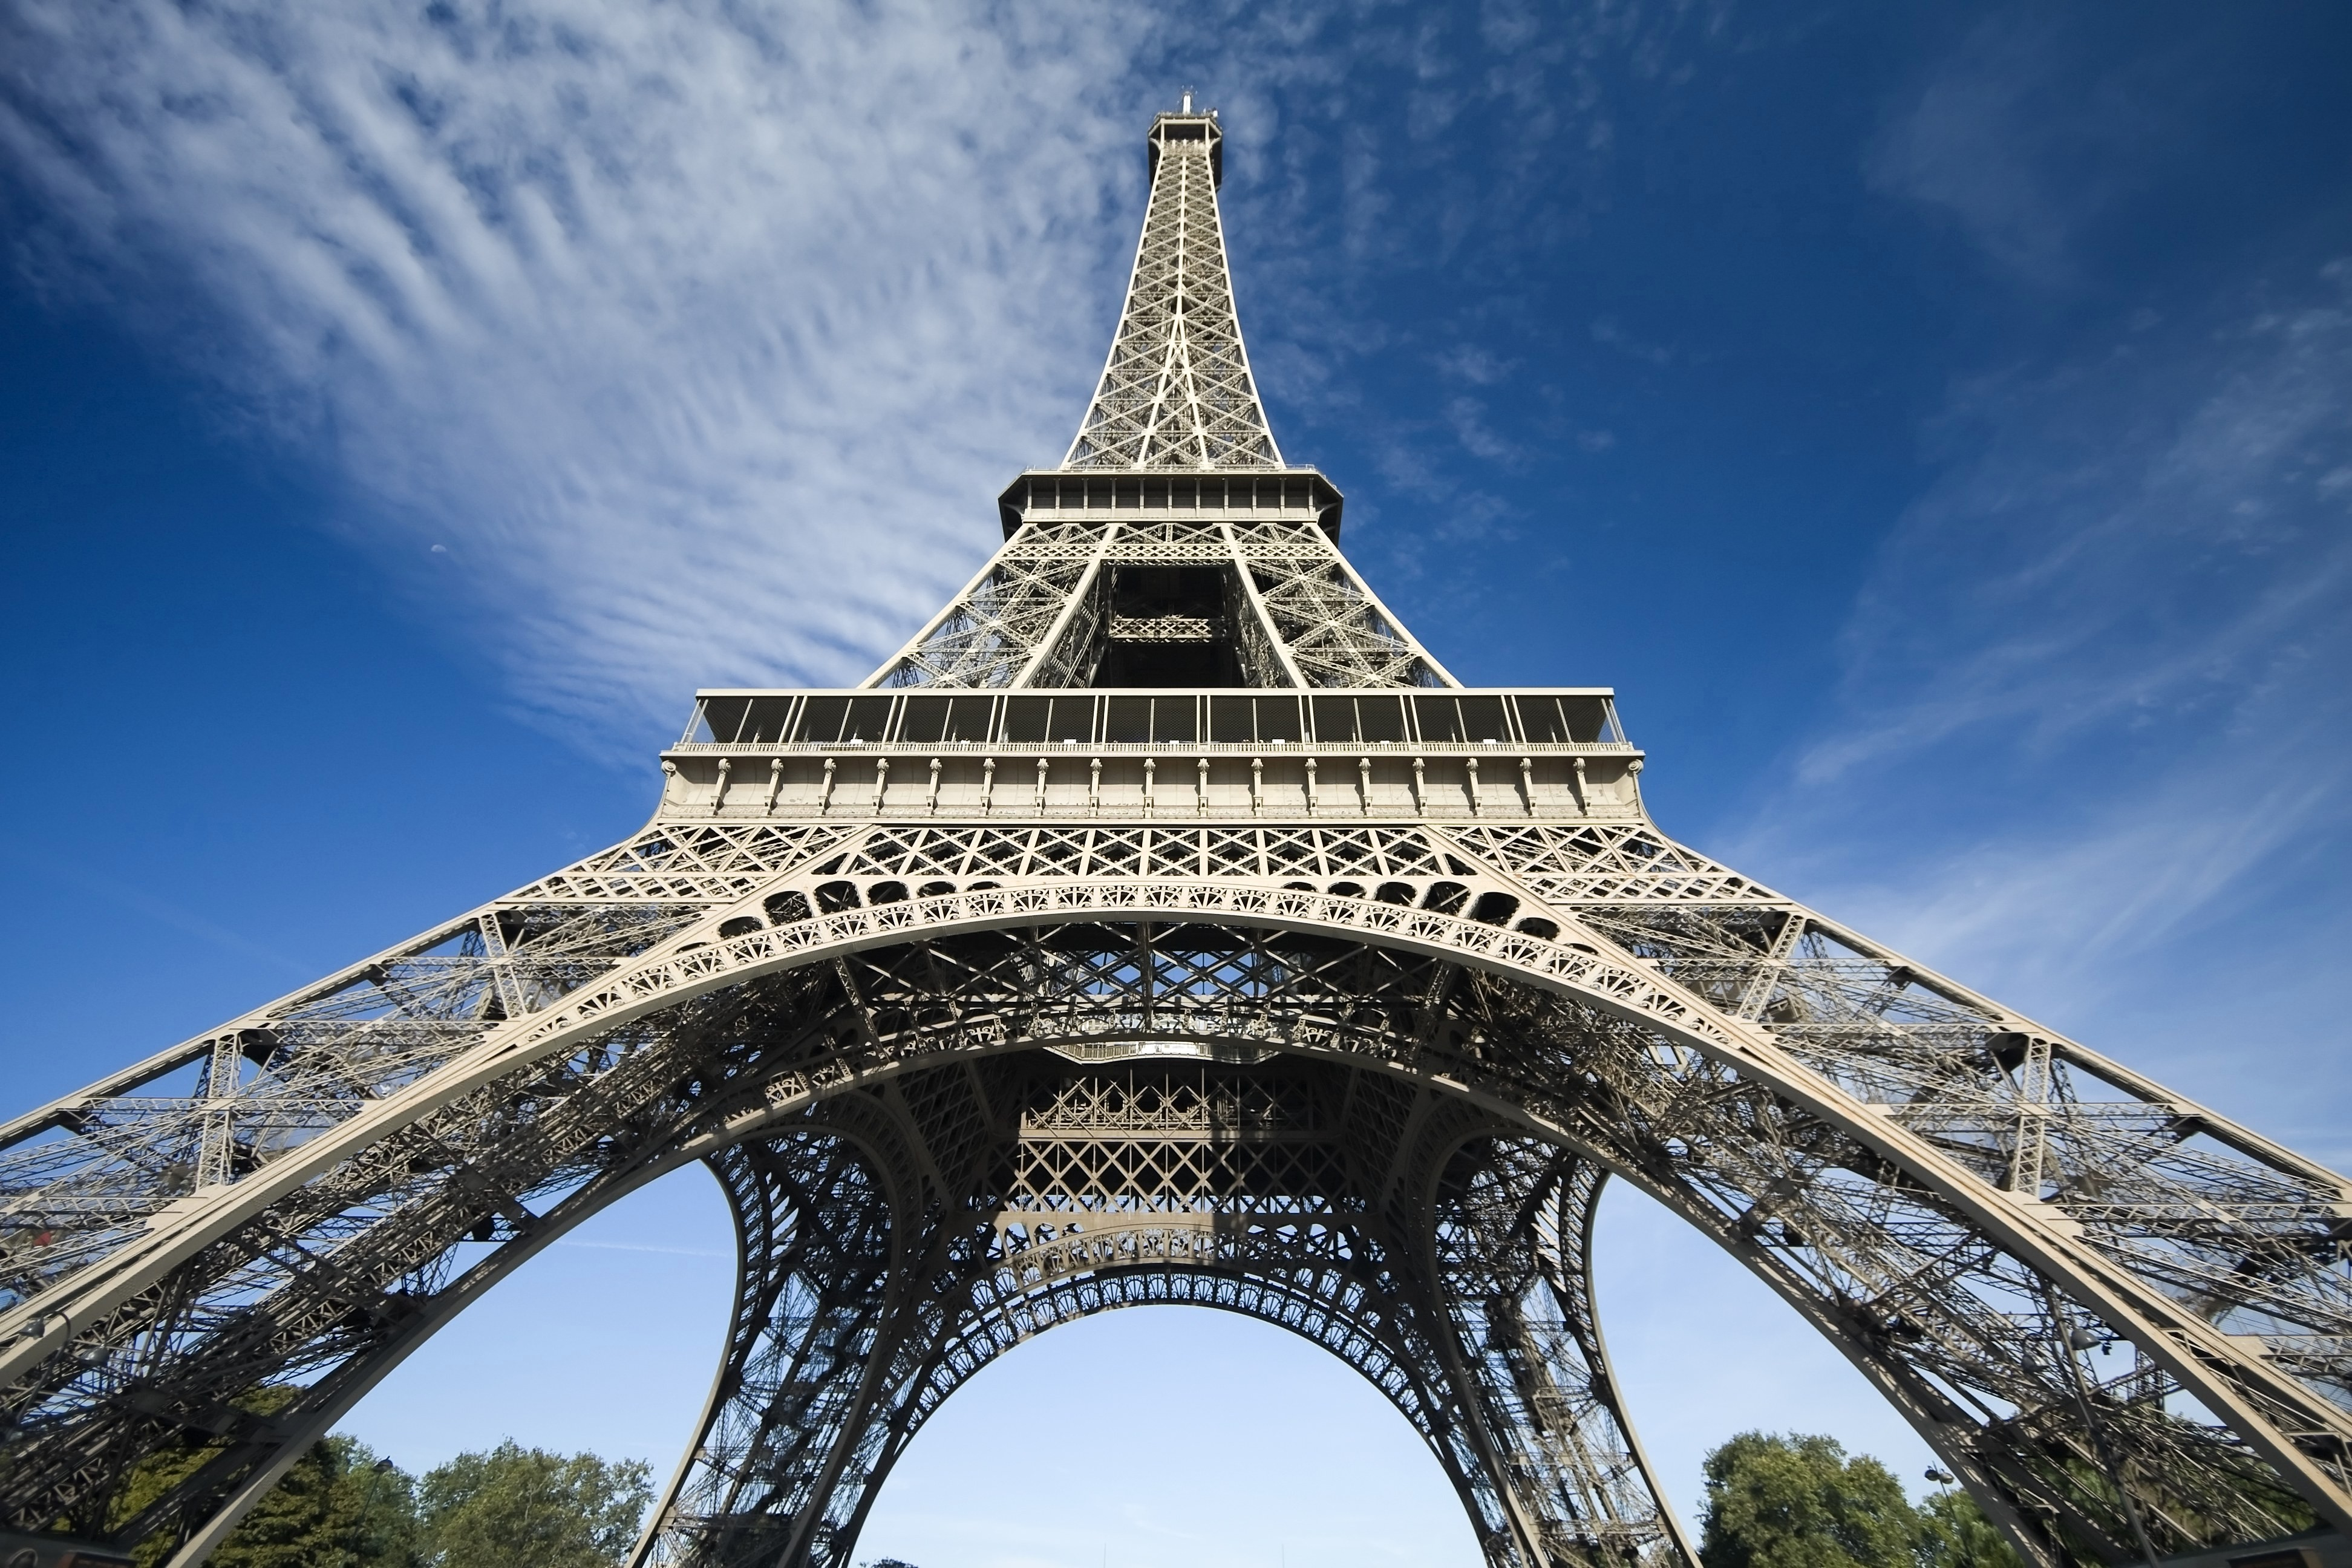
\includegraphics[width=\linewidth]{./img/out.jpg}
    \caption{Image after conversion}
  \end{subfigure}
\end{figure}

\end{document}
